\documentclass[9pt]{book}
%\usepackage[spanish]{babel}
\usepackage{fancyhdr}
\usepackage{color}
\usepackage[latin1]{inputenc}
\usepackage{indentfirst}
\usepackage{graphicx}
\usepackage{graphicx}
\graphicspath{ {./imagenes/} }
%\usepackage{rotating}
\usepackage{amssymb}
\usepackage{amsmath}
%\usepackage{shapepar}
%\usepackage[small]{caption}
%\usepackage{lscape}
%\usepackage{natbib}
\pagestyle{fancy}
%\usepackage{mathrsfs}
%\usepackage{multirow}
\newcommand{\ihat}{\mathbf {\hat \imath}}
\newcommand{\jhat}{\mathbf {\hat \jmath}}

%\renewcommand{\chaptermark}[1]{\markboth{#1}{}}
%\renewcommand{\sectionmark}[1]{\markright{\thesection\ #1}}
%\lhead[\fancyplain{}{\bfseries\thepage}] {\fancyplain{}{\bfseries\rightmark}}
%\rhead[\fancyplain{}{\bfseries\leftmark}] {\fancyplain{}{\bfseries\thepage}}
%\cfoot{}
%\newcommand{\ud}{\;\mathrm{d}}
%\renewcommand{\sin}{\mbox{\,sen\,}}
%\renewcommand{\tablename}{Tabla}
%\setlength{\captionmargin}{19pt}
%\renewcommand{\captionlabelfont}{\sffamily}
%\renewcommand{\labelenumi}{(\arabic{enumi})}
% Para que no ponga encabezados en hojas vacias
%\newcommand{\clearemptydoublepage}{\newpage{\pagestyle{empty}
%            \cleardoublepage}}
% Para que incluya en el ap\'endice resumen, introducci\'on, etc.
%\newcommand{\capitulo}[1]{\chapter*{#1}
%              \addcontentsline{toc}{chapter}{#1}
%               \markboth{\MakeUppercase { #1 } }{\MakeUppercase { #1 } }}



\begin{document}

\numberwithin{equation}{chapter}
  \renewcommand{\thepage}{\arabic{page}}
  \setcounter{page}{1}
  \renewcommand{\tablename}{Tabla}

 \chapter{Introducci\'on}


Desde tiempos antiguos el Sol ha sido estudiado para cosas como la predicci\'on de las estaciones del a\~no, que si bien a\'un nos es \'util, hoy en d\'ia esta estrella tiene un impacto a\'un m\'as fuerte en nosotros, debido a la infraestructura aeroespacial y las telecomunicaciones de las que tanto dependemos. La estructura de la atm\'osfera solar como funci\'on de temperatura ha sido un problema complicado para la investigaci\'on de la f\'isica solar \cite{VAULT1}, por lo que realizar un modelo preciso para el comportamiento Solar es hasta ahora imposible. Es por esto que el estudio del estado fisico de la atm\'osfera solar conlleva a importantes cuestionamientos y avances en la descripci\'on del modo en c\'omo se genera y se transporta energ\'ia a trav\'es de \'esta.

La atm\'osfera solar se extiende desde los niveles fotos\'ericos hasta el medio coronal pasando por el medio cromosf\'erico, involucrando un rango de longitud de 1\(R_\odot\) -- 3\(R_\odot\), y est\'a descrita b\'asicamente por la f\'isica de un plasma magnetizado. El estado del plasma y/o su interacci\'on con el campo magn\'etico establecen mecanismos de emisi\'on en pr\'acticamente todo el espectro electromagn\'etico. Estos mecanismos consisten en trancisiones at\'omicas (que pueden ser ionizantes, de recombinaci\'on y tipo ligado-ligado) y mecanismos de emisi\'on libre-libre como radiaci\'on \emph{bremsstrahlung} y radiaci\'on sincrotr\'onica.

La \emph{fot\'osfera} se consiste en granulos convectivos de peque\~na escala ($10^3$~km), separados de entre s\'i por capas intergranulares, las cuales concentran elementos de alto flujo magn\'etico ($|B| \le 1\mbox{kG}$). La escala temporal de la ocurrencia de un gr\'anulo es de unos minutos aproximadamente. La \emph{crom\'osfera} es una capa que se extiende por alrededor de $2\times 10^3$~km y emite copiosamene en la l\'inea espectral H$\alpha$ ($\lambda=6563~\AA$) y ultravioleta. Similarmente a la fot\'osfera, la base de la crom\'osfera presenta gr\'anulos con una escala de tama\~no relativamente mayor concentrando flujo magn\'etico, el cual est\'a asociado con flujos verticales de plasma llamados \emph{esp\'iculas}. M\'as all\'a de la base de la crom\'osfera cambia la condici\'on en la presi\'on dominante, ya que mientras la presi\'on del gas domina a niveles fotosfericos, a estos niveles esta condici\'on se invierte y las distribuciones de brillo observadas est\'an dominadas por la geometr\'ia del campo magn\'etico.

El efecto de estas micro r\'afagas podr\'ia ser utilizado como parte de la explicaci\'on para el cambio tan dr\'astico de temperatura entre la crom\'osfera y la corona solar, lo cu\'al podr\'ia ser un gran paso hacia comprender mejor la atm\'osfera solar.

Las temperaturas implicadas en este cambio de morfolog\'ia, de gr\'anulos a estructuras filamentarias magn\'eticas (\emph{loops}) es de $2\times 10^5~\mbox{K} < T < 10^6~\mbox{K}$ proponiendo que, a trav\'es de las ep\'iculas se establece un mecanismo continuo de transferencia de material y energ\'ia hacia la corona solar, por lo que se han propuesto modelos que expliquen la din\'amica y estructura t\'ermica de una condici\'on conocida como \emph{Sol Quieto}, en referencia a regiones del Sol que exentas de cualquier manifestaci\'on de actividad observable. Modelos est\'aticos de atm\'osferas referentes, han sido desarrollados por Vernazza et al. 1991 (VAL)\cite{VAULT1}, Fontenla et al. 1993 y Avrett y Loeser 2008 (C7) \cite{C7}). En ellos, se ajusta una atm\'osfera hidrost\'atica, promediando propiedades estratificadas, y con aproximaci\'on plano-paralela, hasta reproducir el correspondiente espectro emergente para un conjunto de observaciones seleccionadas. A\'un cuando la f\'isica de aquellos modelos es bastante realista, no toma en cuenta la din\'amica a escala angular menor al poder de resoluci\'on de las observaciones comparadas con los modernos instrumentos de hoy. 

Si bien, en comparaci\'on con los modelos din\'amicos mencionados arriba, los modelos est\'aticos han sido escasamente estudiados, y es eso en lo que se enfoca este trabajo. Aqu\'i realizamos una extensi\'on del programa \emph{PakalMPI} (De la Luz 2010) (c\'odigo que resuelve la ecuaci\'on de transferencia radiativa en tres dimensiones en una aproximaci\'on plano-paralela, cuya estratificaci\'on sigue perfiles conocidos de densidad y temperatura), y se agrega una aproximaci\'on del efecto de los campos magn\'eticos a la ecuaci\'on de estado para intentar realizar un c\'alculo m\'as realista a la estructura de la crom\'osfera.

\section{Estructuras de micro-escala en la cromosfera solar}
%Esto lo dijo victor
observaciones de la red cromosfericas y del experimento VAULT.
%

Con el advenimiento de instrumentos que observan en el rango UV, tales como IRIS (Interface Region Imaging Spectrograph) se observa que la estructura de la atm\'osfera (y muy particularmente, de la crom\'osfera) contienen una distribuci\'on ca\'otica y que un modelo que promedie propiedades (como val C o C7 no puede capturar la complejidad del escenario real.

Carlsson y Sten (1994) modelan bidimensionalmente la emisi\'on emergente t\'ermica libre-libre a cromosf\'erica longitudes de onda milim\'etricas y sub-milim\'etricas. La temperatura de brillo resultante var\'ia sensiblemente en el tiempo debido a la propagaci\'on de ondas de choque y modos de oscilaci\'on, contabilizando una complejidad m\'as realista para la temperatura local del gas en las capas de formaci\'on del continuo de emisi\'on. Las escalas angulares involucradas en estos resultados est\'an por debajo de los 0.1''. Asi, la emisi\'on milim\'etrica y submilim\'etrica dependen fuertemente. Loukitcheva et al. 2004 refieren que las el escenario din\'amico de la estructura cromosf\'erica es consistente con la emisi\'on milim\'etrica y submilim\'etrica observada.




Cuando observamos el sol, existe una capa muy brillante, conocida como fot\'osfera, la cu\'al debido a su intensidad de brillo enmascara las emisiones del resto de las regiones solares, sin embargo, cuando la luz de la fot\'osfera es filtrada, el resto de las regiones m\'as d\'ebiles desaparecen tambi\'en por completo, por lo que solo durante un eclipse solar es posible apreciar el resto de las capas del sol.

Por encima de la fot\'osfera, y extendi\'endose acerca de 5,000km por arriba de su superficie turbulenta, encontramos una regi\'on de la am\'osfera llamada crom\'osfera. El color de esta regi\'on es debido a una alta emisi\'on en la l\'inea de hidr\'ogeno (H-alpha) y la l\'inea K (CaII K - de los \'atomos de calcio con un eletr\'on removido), y aunque la mayor emisi\'on proviene de estas l\'ineas, tambi\'en existe emisi\'on en el cont\'inuo y en las principales l\'ineas de Pashen y Balmer.  Esta regi\'on solo es posible observarla durante eclipses solares con telescopios sofisticados y es de un color rojizo que es por lo que se le da el nombre de crom\'osfera (cromo - esfera). En esta regi\'on la temperatura va aproxim\'adamente de 6,000°C a 20,000°C.  

Cuando el sol es observado por medio de un espectr\'ografo o alg\'un filtro que aisle la emisi\'on H-alpha, se logran observar nuevas caracter\'isticas. Entre estas se encuentran la red cromosf\'erica de elementos de campo magn\'etico. Esta red describe las c\'elulas super granulares y es debido a la presencia de conjuntos de l\'ines de campo magn\'etico ah\'i concentradas. Esta red rodea las celdas super granulares y esto debido a la presencia de los conjuntos de l\'ineas de campo magn\'etico ah\'i concentradas por el movimiento de flu\'ido en los supergr\'anulos.

%En la figura \ref{fig:chromosphericnet} se observa una imagen tomada en la l\'inea de c\'alcio de la red cromosf\'erica, mientras que en la figura 

\begin{figure}[h]
\caption{"Fuente: The Chromospheric Network Mayo 2017, NASA webpage oficial"}
\centering
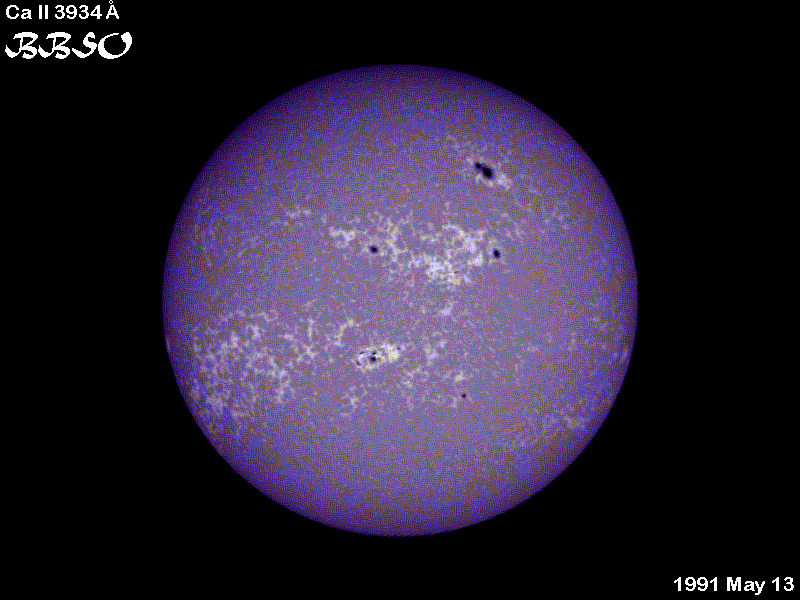
\includegraphics[scale=0.3]{CAII3934}
\label{fig:chromosphericnet}
\end{figure}



\section{El c\'odigo \emph{PakalMPI}}
Descripci\'on del c\'odigo, puntualmente hay qu\'e explicar primero para qu\'e sirve actualmente y a partir de ello, plantear las modificaciones.


\chapter{Emisi\'on submilim\'etrica solar}
Mecanismos de la emisi\'on milim\'etrica del plasma del sol quieto, antecedente hist\'orico y enfoque del problema a resolver (qu\'e se va a hacer, por qu\'e se va a hacer y c\'omo se va a a hacer)
  
\chapter{Modelo de Micro estrucras magneticas solares}
\section{Caracteristicas Fisicas}
Aqui van las propiedades fisicas de los modelos que vamos a implementar. Por ejemplo, definir las escalas de altura, las intensidades de campo, temperatura, densidades, etc.

Para llevar a cabo la simulaci\'on del comportamiento de los campos magn\'eticos se utilizaron dos modelos distintos; uno en forma de arcos magn\'eticos \cite{loops} y otro en forma de un flujo emergente \cite{flujoemergente}.

La primer aproximaci\'on para el modelo de campo magn\'etico fue el de un loop con forma semi-circular, el cu\'al puede ser modelado como un campo magn\'etico dipolo generado por un cable dipolo enterrado debajo de la fo\'sfera.
En este modelo es posible calcular las tres componentes del campo magn\'etico por medio de las siguientes ecuaciones \citation{Jackson}:

\begin{equation}
    B_r(r,\theta)=\frac{2mcos\theta}{r^3}
\end{equation}
  
\begin{equation}
    B_\theta(r,\theta)=\frac{2msin\theta}{r^3}
\end{equation}

\begin{equation}
    B_\phi(r,\theta)=0
\end{equation}

Donde m representa el momento magn\'etico inducido por el anillo de corriente I con un conductor de radio a, y los par\'ametros theta y r son los par\'ametros libres que movemos para ir generando los valores del campo.

Para la segunda aproximaci\'on del modelo se consider\'o un flujo emergente, ya que una gran cantidad del flujo magn\'etico en la fot\'osfera solar consiste en fuertes campos en elementos no resueltos. Este modelo consiste en un elemento magn\'etico con una simetr\'ia de un tubo de flujo cil\'indrico incrustado en la fot\'osfera.

Los valores de sus componentes son calculados como

\begin{equation}
B_z(r,z)=B_z(0,z)D(\alpha)
\end{equation}

\begin{equation}
B_r(r,z)=-\frac{1}{2}r\frac{dB_z(0,z)}{dz}D(\alpha)
\end{equation}

Este campo satisface gradiente $ \nabla \cdot B = 0 $. La funci\'on radial $D(\alpha)$ es tomada como
\begin{equation}
 D(\alpha) = 
    \begin{cases}
        (1-alpha^2)^2 & \alpha \leq 1 \\
        0   & \alpha > 1
    \end{cases}
\end{equation}

donde $\alpha = r/r_0(z)$. El radio $r_0(z)$ del tubo a una altura z es promediado a lo largo del c\'irculo de radio R que es obtenido de:

\begin{equation} \label{r_flujo_emergente}
r_0^-2(z) = \frac{2\pi B_z(0,z)}{\phi} \int_{0}^{1} \alpha D(\alpha) d\alpha = \frac{\pi B_z(0,z)}{3 \phi}
\end{equation}

donde $\phi$ es el flujo magn\'etico dentro del tubo.
El campo axial es considerado

\begin{equation}
B_z(0,z)=B_0e^{\frac{-z}{h}}
\end{equation}

Por lo tanto la fuerza axial de campo es $B_0$ en el origen $z=0$ que en nuestro caso se ubica al nivel de la fot\'osfera (CORRIGEME). En este modelo el campo diverge a diferente ritmo dependiendo de la escala de altura h.

Conforme $h\rightarrow \infty , B_z(0,z) \rightarrow B_0$, $a$ constante, y por la ecuaci\'on \ref{r_flujo_emergente} $r_0(z) \rightarrow r_0 = (3\phi / \pi B_0)^\frac{1}{2}$, es tambi\'en una constante.

En los c\'alculos consideramos $\phi=2.8x10^18$Mx y $B0=2000$Gauss. Esto implica tubos de flujo de 366km a $Z=0$


\section{Implementaci\'on del modulo para Magnetohidrost\'atica}
Aqui va la info de como implementaste los modelos.


\chapter{Resultados}
\section{Micro arco magnetico}
resultados de las simulaciones para el modelo de arcos magneticos
\section{Flujo emergente}
resultados de las simulaciones para flujo emergente


\chapter{Discusi\'on y conclusiones}
Comparaci\'on entre ambos modelos, discusion y resultados
hola Springer Science \& Business Media, Aug 26, 2006

\begin{thebibliography}{9}

\bibitem{VAULT1} 
A. Vourlidas, B. Sanchez, E. Landi, et al.
\textit{The structure and Dynamics of the Upper Chromosphere and Lower Transition Region as Revealed by the Subarcsecond VAULT Observations, Astronomy and Astrophysics} 
Solar Physics, 2010.

\bibitem{VALC}
J. E. Vernazza, E. H. Avrett y R. Loeser
\textit{Structure of the Solar Chromosphere. III. Models of the EUV Brightness Components of the Quiet Sun} 
The Astrophysical Journal Supplement Series, 1981.

\bibitem{C7}
J. M. Fontenla, E. H. Avrett y R. Loeser
\textit{Energy Balance in the Solar Transition Region. I. Hydrostatic Thermal Models with Ambipolar Difussion} 
The Astrophysical Journal, 1990.

\bibitem{loops} 
Markus Aschwanden. 
\textit{Physics of the Solar Corona} 
Springer Science \& Business Media, 2006.

\bibitem{flujoemergente} 
Rees and Seemel.
\textit{Line Formation in an Unresolved Magnetic Element: A Test of the Centre of Gravity Method} 
Astronomy and Astrophysics, 1978

\bibitem{Jackson} 
A. Vourlidas, B. Sanchez, E. Landi, et al.
\textit{Classical Electrodynamics} 
John Wiley and Sons, 1962.


\end{thebibliography}


\end{document}    </include>
    </context>

    <context id="math-2" style-ref="math" class="no-spell-check">
      <start>\\\[</start>
      <end>\\\]</end>
      <include>
        <context sub-pattern="0" where="start" style-ref="math-boundary"/>
        <context sub-pattern="0" where="end" style-ref="math-boundary"/>
        <context ref="in-math"/>
      </include>
    </context>

    <context id="math-env" style-ref="math" style-inside="true" class="no-spell-check">
      <start>(\\begin)\{(math|displaymath|equation\*?|align\*?|eqnarray\*?)\}</start>
      <end>(\\end)\{\%{2@start}\}</end>
      <include>
        <context sub-pattern="1" where="start" style-ref="common-commands"/>
        <context sub-pattern="1" where="end" style-ref="common-commands"/>
        <context ref="in-math"/>
      </include>
    </context>

    <context id="inline-math-1" style-ref="inline-math" class="no-spell-check">
      <start>\$</start>
      <end>\$</end>
      <include>
        <context sub-pattern="0" where="start" style-ref="math-boundary"/>
        <context sub-pattern="0" where="end" style-ref="math-boundary"/>
        <context ref="in-math"/>
      </include>
    </context>

    <context id="inline-math-2" style-ref="inline-math" class="no-spell-check">
      <start>\\\(</start>
      <end>\\\)</end>
      <include>
        <context sub-pattern="0" where="start" style-ref="math-boundary"/>
        <context sub-pattern="0" where="end" style-ref="math-boundary"/>
        <context ref="in-math"/>
      </include>
    </context>

    <context id="math">
      <include>
        <context ref="math-1"/>
        <context ref="math-2"/>
        <context ref="math-env"/>
        <context ref="inline-math-1"/>
        <context ref="inline-math-2"/>
      </include>
    </context>

    <context id="latex">
      <include>
        <context ref="comment"/>
        <context ref="verbatim"/>
        <context ref="R-block"/>
        <context ref="headings"/>
        <context ref="math"/>
        <context ref="urls"/>
        <context ref="specific-commands"/>
        <context ref="common-commands"/>
        <context ref="special-char"/>
        <context ref="gen
